\makeatletter
\def\input@path{{../}}
\makeatother
\documentclass[../main.tex]{subfiles}
\graphicspath{
  {"../images/03/"}
  {"./images/03/"}
}

\begin{document}
\chapter{Probability Distributions}
\section{Random Variables}
\begin{definition}
A \textbf{random variable} is a function $X : \Omega \rightarrow R$. It assigns a real number to each outcome. 
\end{definition}
(In other words, a random variable is like a vending machine- it dispenses numbers according to a possibly unknown function.)

A random variable $X$ might output some concrete number $x$, with some probability. If this probability is $\frac 12$, then we write this
\[
	\Pr[X = x] = \frac 12
\]
For the sake of continuing the ``vending machine'' analogy, we will temporarily say \[\Pr[X \hookrightarrow x] = \frac 12,\] where $\hookrightarrow$ is pronounced ``dispenses,'' i.e. $X$ dispenses $x$ with probability $\frac 12$. 
\section{Discrete Random Variables}
\subsection{Probability Mass Function}

These random variables have probabilities associated with them, just as
outcomes and events in the sample space. The probability function
associated with a discrete random variable is called a \textbf{probability
mass function}
\begin{definition}
    A \textbf{probability mass function} (pmf) is a function  $f:\RR \rightarrow [0,1]$ from the reals to the unit interval such that $f(x) = \Pr[X \dsp x]$, that is the probability that
    a random variable dispenses a given value. It must satisfy the following criteria
    \begin{enumerate}
        \item $\displaystyle \sum_{x_i} f(x_i) = 1$, where the sum is over
        every $x_i$ in the range of $X$.
        \item $f(x_i) = 0$ for every $x_i$ not in the range of $X$.
    \end{enumerate}
\end{definition}
We will elucidate these ideas with a number of examples
\begin{example}
    Let a 6-sided die be constructed such that the probability of rolling
    a 4 is twice that of rolling any other value. Describe this in terms
    of a random variable $X$ and a pmf $f(x)$. Next, let $Y$ be the number of
    prime factors of $X$. Give the pmf of $Y$.
\end{example}
\begin{solution}
Let $X$ be a random variable that dispenses the value the die shows (in $1, 2, \ldots 6$). $f(x)$ is a function such that $f(1) = f(2) = f(3) = f(5) = f(6) = \frac{1}{7}$, $f(4) = \frac 27$, and $f(x)$ is 0 otherwise. 

Suppose $Y$ is the number of prime divisors of $X$. We can calculate what $Y$ outputs for given values that $X$ outputs: 
\begin{center}\begin{tabular}{c|c}
     X & Y \\ \hline 
     1 & 0\\
     2 & 1 \\
     3 & 1 \\
     4 & 1 \\
     5 & 1 \\
     6 & 2 
\end{tabular}
\end{center}
This means that for the pmf of $Y$, $g(y)$, $g(0) = \Pr[Y=0] = \frac 17$, $g(1) = \Pr[Y=1] = \frac 57$, $g(2) = \Pr[Y=2] = \frac 17$, and $g(y) = 0$ otherwise. 
\end{solution}

\begin{example}
Let $X$ be the sum of the pips showing on 2 rolled, fair, 10-sided die.
Find the pmf for $X$.
\end{example}

\begin{solution}
The \textbf{support set} of $X$, or the set of possible values of $X$, is $\{ 2, 3, \ldots 20 \}$, so we can write out a few values of $f$: 
\[
    f(2) = \frac{1}{100}, \quad f(3) = \frac{2}{100}, \quad \ldots \quad f(20) = \frac{1}{100}
\]
We can write out a nice closed form for $f$: 
\begin{center} $f(x) = 
    \begin{cases}
        \frac{10 - |11-x|}{100} & x \in \{2, 3, \ldots 20 \} \\
        0 & \text{otherwise}
    \end{cases}$
\end{center}
\end{solution}

\begin{example}
5 Juniors and 5 seniors take a test and are ranked 1-10 according to their
test score (1 = highest score). Assume all scores are distinct and that all $10!$ student rankings are equally likely. Let $X$ be the highest rank (smallest
integer value) of a junior in the class. Find the pmf $f(x)$ for $X$.
\end{example}
\begin{solution}
There are $\binom{10}{5}$ ways to arrange the seniors and juniors into distinct ranking orders. To calculate the individual values of $f$, we proceed with casework. 

\textbf{If $X$ = 1}, a junior must have taken the highest rank, and then the remaining juniors and seniors can fill in the ranks in any order. This can be accomplished in $\binom{9}{4}$ ways, so $f(1) = \frac{\binom{9}{4}}{\binom{10}{5}} = \frac 12$. 

\textbf{If $X$ = 2}, a senior takes rank 1, a junior takes rank 2, and the remaining juniors and seniors can fill in the rest of the ranks. This can be accomplished in $\binom{8}{4}$ ways, so $f(2) = \frac{\binom{8}{4}}{\binom{10}{5}} = \frac{5}{18}$. 

A similar analysis can be done for the cases where $X = 3, 4, 5, 6$. The highest rank of a junior can't be lower than 6, as that would require more than 5 seniors to fill in rankings. In general, a closed form could be 
\[
    f(x) = \begin{cases} \frac{\binom{10-x}{4}}{\binom{10}{5}} & x \in \{1, 2, \ldots 6\} \\ 0 & \text{otherwise}. \end{cases}
\]
\end{solution}
\begin{remark}
Note that if we try ensure that the sum of all of the outputs of $f(x)$ is 1, we get a version of the famed \textit{hockey stick identity}: 
\[
    \binom{4}{4} + \binom{5}{4} + \binom{6}{4} + \binom{7}{4} + \binom{8}{4} + \binom{9}{4} = \binom{10}{5}
\]
This can be generalized to arbitrary $r=4, n=9$: 
\[
    \sum_{k=r}^n \binom{k}{r} = \binom{n+1}{r+1}
\]
\end{remark}
\begin{example}
Let $f(0) = f(1)$ and $f(k+1) = \frac{1}{k}f(k)$. If you know
that $f$ is a pmf over the non-negative integers, then find $f(0)$.
\end{example}
\begin{solution}
We write out a few of the first few values of $f(k)$ in terms of $f(0)$: 
\begin{align*}
    f(2) &= f(1) = f(0) \\
    f(3) &= \frac{1}{2} f(2) = \frac 12 f(0)\\
    f(4) &= \frac 13 f(3) = \frac 16 f(0) \ldots 
\end{align*}
In order for the pmf to satisfy $\sum_{x_i} f(x_i) = 1$, we get that 
\begin{align*}
    f(0) + f(1) + f(2) + f(3) + f(4) + \ldots &= f(0) + f(0) + f(0) + \frac{1}{2} f(0) + \frac 16 f(0) + \ldots \\ &= f(0) \left(1 + \sum_{n=0}^\infty \frac{x^n}{n!}\right) \\ &= f(0) (1 + e) = 1
\end{align*}

Therefore, $f(0) = \frac{1}{1+e}$.
\end{solution}
\begin{example}
\label{ex:squarepdf}
Find $k$ if $f(x) = \dfrac{k}{x^2}$ is a pmf over positive integers.
\end{example}
\begin{solution}
In order for the pmf to be valid, we require the pmf to be \textit{normalized}, i.e. $\sum_{x_i} f(x_i) = 1$, so 
\[
    k \sum_{n=1}^\infty \frac{1}{n^2} = 1 = \frac{\pi^2 k}{6} \implies k = \frac{6}{\pi^2}.
\]
\end{solution}
\begin{example}
In Example~\ref{ex:squarepdf}, let $X$ be a random variable over positive
integers with pmf $f$. Let $Y$ be a random variable that equals 1 if $X$ is
even and 2 if $X$ is odd. Find the pmf of $Y$.
\end{example}
\begin{solution}
We can evaluate $g(1)$ and $g(2)$ independently. $g(1)$ is the sum of the probabilities that $X$ dispenses an odd number: 
\[
    g(1) = \sum_{n=0}^\infty \Pr[X = 2n+1] = \frac{6}{\pi^2}\sum_{n=0}^\infty \frac{1}{(2n+1)^2} 
\]
and $g(2)$ is the sum of the probabilities that $X$ dispenses an even number: 
\[
    g(2) = \sum_{n=1}^\infty \Pr[X = 2n] = \frac{6}{\pi^2}\sum_{n=1}^\infty \frac{1}{4n^2} 
\]
This latter sum is easier to evaluate -- it becomes $\frac 14 \cdot \frac{\pi^2}{6} = \frac{\pi^2}{24}$, so $g(2) = \frac{6}{\pi^2} \cdot \frac{\pi^2}{24} = \frac 14$. The sum of squares of odd reciprocals is $\frac{\pi^2}{8}$, so $g(1) = \frac 34$, which is perfectly consistent. 
\end{solution}
\begin{example}
Find $k$ if $f(x) = \dfrac{k}{x}$ is a pmf over positive integers.
\end{example}
\begin{solution}
This is not a valid pmf -- in trying to normalize the pmf, we require
\[
    \sum_{n = 1}^\infty \frac{k}{n} = 1,
\]
but the left hand side of the equation diverges. Such a pmf does not exist. 
\end{solution}
\subsection{Cumulative Mass Functions}
A probability mass function over a random variable $X$ gives the probability 
that $x$ equals a certain value. In many instances it will prove quite helpful 
to work with instead the probability that $X$ is less than or equal to a 
certain value. This is called the \textit{cumulative mass function}.
\begin{definition}
The \textbf{cumulative mass function (cmf)} of a random variable $X$ with 
pmf $f$ is defined as a function $F: \RR\rightarrow[0,1]$ such that
$$F(x) = \Pr[X \leq x] = \sum_{-\infty}^x f(t)$$
\end{definition}
\begin{example}Let $X$ be the sum of the pips on the roll of 2 fair six-sided
die. Find the cmf of $X$.
\end{example}
\begin{solution}
It is impossible to have a sum of 1 or less on two dice rolls, so $F(1) = 0$. We calculate $F(2)$ by noting the only non-zero contribution is if two 1's show up on both of the dice, so $F(2) = \Pr[X \leq 2] = f(2) = \frac{1}{36}$. Similarly, $F(3) = \Pr[X \leq 3] = f(2) + f(3) = \frac{1}{36} + \frac{2}{36} = \frac{3}{36}$, and $F(4) = \Pr[X \leq 4] =  f(2) + f(3) + f(4)= \frac{1}{36} + \frac{2}{36} + \frac{3}{36} = \frac{6}{36}$. We can continue computing in this way until we eventually reach $F(11) = \displaystyle\sum_{k=1}^{11} f(k) = 1-f(12) = \frac{35}{36}$. See Figure~\ref{fig:cmf_dice} for a graph of the cmf -- note how it monotonically increases until it reaches a final maximum value at 1. 
\begin{figure}
	\centering
	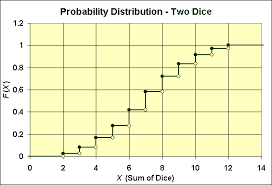
\includegraphics[width=0.7\linewidth]{cmf_dice.png}
	\caption{Cumulative distribution function for the sum obtained by rolling two dice}
	\label{fig:cmf_dice}
\end{figure}

\end{solution}
\begin{example}
Let $f(x) = c\left(\dfrac{1}{4}\right)^x$ be the pmf of the random variable $X$, where the support set is $\ZZ_{\geq 0}$ 
\begin{enumerate}
\item Find the appropriate constant $c$
\item Determine the cmf $F(x)$
\item Use the cmf to compute $\Pr[2 < X \leq 8]$
\item Write formulas involving $F$ and $f$ for the following
    \begin{enumerate}
        \item $\Pr[X > a]$
        \item $\Pr[X \geq a]$
        \item $\Pr[a < X < b]$
        \item $\Pr[a \leq X \leq b]$
    \end{enumerate}
\end{enumerate}
\begin{solution}
Most of the following analysis follows from definition: 
\begin{enumerate}
    \item Using the sum of an infinite geometric series formula, we arrive at $c = \frac 34$. 
    \item Using the sum of a finite geometric series formula, we arrive at $F(x) = \frac{3}{4}\left(\frac{1-(1/4)^{x+1}}{1-1/4}\right) = 1-(1/4)^{x+1}$
    \item $\Pr[2 < X \leq 8] = F(8)-F(2) = \frac{4095}{262144}$, from the cmf in b
    \item This is a more general question that applies to other cmfs other than this one: 
    \begin{enumerate}
        \item $\Pr[X > a] = 1-F(a)$
        \item $\Pr[X \geq a] = 1-F(a)+f(a) = 1-F(a)+\displaystyle\lim_{\Delta t \to 0} (F(a)-F(a-\Delta t))$
        \item $\Pr[a < X < b] = F(b)-F(a)-f(b) = F(b)-F(a)-\displaystyle\lim_{\Delta t \to 0} (F(b)-F(b-\Delta t))$
        \item $\Pr[a \leq X \leq b] = F(b)-F(a)+f(a)=F(b)-F(a)+\displaystyle\lim_{\Delta t \to 0} (F(a)-F(a-\Delta t))$
    \end{enumerate}

    % remark: the cmf is like the ``integral'' of f, if a ``derivative'' of F gives f?
\end{enumerate}
\end{solution}
\begin{remark}
Please note that what we are calling the cmf is very often called a \textbf{distribution function} in other texts and even by us, later on. The reasons will become more apparent when we extend pmf and cmf to continuous functions and partly-continuous functions.
\end{remark}
\end{example}

\subsection{Discrete Joint Probability Functions}

When two or more random experiments occur simultaneously, the 
outcomes can be analyzed with the use of a \textit{joint probability
function}. A common example is the height, $X$,  and weight, $Y$, of randomly selected subjects. If the subjects are humans, the sample space of $X$ (in feet) could 
be $\Omega_X = [0,10]$ and weight $\Omega_Y = [0,1000]$ in pounds.\footnote{These
sample spaces are discrete technically because of the finite limitation
of measurement, but for all practical purposes would best be treated as
continuous. The type doesn't concern us here; it's still a nice example.}

If enough sample data were collected, one could approximate $\Pr[X \dsp x \cap Y \dsp y]$ for $(x,y)$ in the joint sample space $\Omega_X \times
\Omega_Y$. This probability defines the joint probability function, or joint pmf:
$$f(x,y) = \Pr[X \dsp x, Y \dsp Y]$$
where the "comma" in the probability implies intersection and is usually read as "and." Be careful to \textbf{not} equate this with $\Pr[X \dsp x]\cdot\Pr[Y \dsp y]$, which would equal $\Pr[X \dsp x, Y \dsp Y]$
only when $X$ and $Y$ are independent. In fact, we should all be able to agree that height and weight of humans (or any type of object) are
almost always correlated and, therefore, \textit{not} independent.

The joint pmf of a set of discrete random variables $\{X_1, \ldots, X_n\}$
satisfies the following properties:
\begin{theorem} If $f$ is a function then $f$ can be the pmf of a set of random variables if and only if
\begin{eqnarray}
     f(x_1,\ldots,x_n) &\geq& 0 \\
    \sum_{x_1}\cdots\sum_{x_n}f(x_1,\ldots,x_n) &=& 1
\end{eqnarray}
Where in both items the sum is taken over all values in the domain of $f$.
\end{theorem}

\begin{example}
Let $f(x,y) = kxy$ be a pmf for $x=1,2,3$ and $y=1,2,3$. Determine the value of $k$.
\end{example}
\begin{solution}
In order to normalize this joint pmf, we force $\displaystyle\sum_x \displaystyle\sum_y kxy = 1$. We can ``pull apart'' the sum: 
\[
    k \left( \sum_x x\right) \left( \sum_y y \right) = 1 \implies k \cdot 6 \cdot 6 = 1 \implies k = \frac{1}{36}.
\]
\end{solution}
\begin{example}
A jar contains 3 red, 2 green and 4 blue marbles. Two marbles are drawn simultaneously at random. Let $R$ be the number of red and $G$ the number
of green marbles drawn. Determine the joint pmf $f(r,g)$
\label{ex:jar}
\end{example}
\begin{solution}
In this case, $R$ can be $0, 1, 2$, and $G$ can be $0, 1, 2$ as well, but these can't be satisfied simultaneously -- in particular, $R$ and $G$ cannot both dispense 2 at the same time. 

To calculate this, we could consider this case-by-case, starting with $\Pr[R=0, G=0]$, say. The probability in this case is 
\[
    f(0,0) = \frac{\binom{3}{0} \binom{2}{0} \binom{4}{2}}{\binom{9}{2}}
\]
and in general, $f(r, g)$ has a closed form: 
\[
    f(r,g) = \frac{\binom{3}{r} \binom{2}{g} \binom{4}{2-r-g}}{\binom{9}{2}}
\]
\end{solution}
\begin{example}
Given the pmf $f(x,y,z)$ of random variables $X,Y,Z$
$$f(x,y,z) = \frac{(x+y)z}{63}\qquad x=1,2; y=1,2,3; z=1,2$$
calculate $\Pr[X \dsp 2, Y+Z \leq 3]$.
\end{example}
\begin{solution}
We can compute this probability by casework. The only possible triples $(x,y,z)$ that work are $(2,1,2)$, $(2,2,1)$, and (2,1,1). If we plug in directly, we get the total probability as 
\[
    \frac{(2+1)2}{63} + \frac{(2+2)1}{63} + \frac{(2+1)1}{63}  = \frac{13}{63}
\]
\end{solution}
The last example hints at a definition for the cumulative
distribution function for a pmf $f$. In the bivariate case the definition is
\begin{definition}
Let $f(x,y)$ be the pmf of two random variables $X$ and $Y$. Then the distribution function $F(x,y)$ is defined by
$$F(x,y) = \Pr[X \leq x, Y \leq y] = \sum_{u=-\infty}^x \sum_{v=-\infty}^y f(u,v)$$
\end{definition}
\begin{example}
Determine the distribution function $F$ for the pmf defined in Example~\ref{ex:jar}. 
\end{example}
\begin{solution}
%% insert the solution here
\end{solution}
\begin{example}
Write an expression for $\Pr[a<X\leq b, c< Y \leq d$] in terms of $F$. %Be 
careful to consider all the cases!
\end{example}
\begin{solution}
It's best to think of this geometrically: 
\end{solution}

\subsection{Marginal and Conditional Distributions}
Marginal distributions and conditional distributions reduce the number of variables in joint distribution functions and d

\begin{definition}
Given $X, Y$, and joint pmf $f(x,y)$, then $f_X(x)$ is the $X$-marginal distribution of $f$, where $f_X(x) = \Pr[X \dsp x]$. 
\end{definition}
We can write out what this means explicitly, in terms of a sum:
\begin{theorem}
\[
    f_X(x) = \sum_y f(x,y)
\]
and 
\[
    f_Y(y) = \sum_x f(x,y)
\]
\end{theorem}
It follows clearly that 
\begin{example}
Consider the following joint distribution function
% X/Y 1 2
% 1 0.4 0.3
% 2 0.2 0.1
Compute the marginal distributions for 
\end{example}

\begin{definition}
Given random variables $X,Y$, and joint pmf $f(x,y)$, the conditional distribution function $f_{X|y}(x|y)$ is equal to 
\[
    f_{X|y}(x|y) = \frac{\Pr[X=x \cap Y=y]}{\Pr[Y=y]} = \frac{f(x,y)}{f_Y(y)}
\]
\end{definition}
This is rather reminiscent of the Law of Total Probability 

\begin{example}
For the joint distribution function above, compute $f_{X|y}(1|Y=1)$.
\end{example}
\begin{solution}[Answer.]
$\frac{0.4}{0.4 + 0.2} = \frac{0.4}{0.6} = \frac{2}{3}$.
\end{solution}

\begin{example}
Suppose we flip a fair coin 4 times. Let $X$ be the number of heads in the first three tosses, and $Y$ be the number of heads in the last three tosses. Find $f(x,y)$, $f_X$, $f_Y$, $f_{X|y}$, and $f_{Y|x}$. 
\end{example}
\begin{solution}
	TBD
\end{solution}
%% insert solution.

\subsection{Exercises}
\begin{enumerate}
	\item Let $f(x,y) = k(x^2+y^2)$ be a pmf for $X,Y$ over the domain $0 \leq x + y \leq 4$
	where $x,y \in \ZZ$.
	\begin{enumerate}
		\item Determine $k$
		\item Calculate $f(1,1)$ and $f(2,3)$
		\item Calculate $f_X(2)$ and $f_Y(1)$
		\item Does $f_X(t) = f_Y(t)$?
		\item Calculate $f_{X|y}(3|y=1)$ and $f_{Y|x}(2|x=2)$
		\item Give a closed-form expression for $f_X(x)$ and $f_{X|y}(x|y)$
	\end{enumerate}
\end{enumerate}
\subsection{Independent Random Variables}

We have already encountered the concept of independent random events. Random variables
are independent when their underlying random processes are independent, and this
can be formalized with properties of the probability mass function. The definition
we will use for independence is that, given two variables $X$ and $Y$, if the outcome
of $Y$ has no effect on the outcome of $X$ then the two variables are independent. 
This is another way of saying the conditional distribution of $X$, conditioned on $Y$
is the same as the distribution of $X$. Formally
\begin{definition}
	Let $X$ and $Y$ be random variables with joint pmf $f(x,y)$. Then $X$ and $Y$
	are \textit{independent} whenever
	$$f_{X|y}(x|y) = f_X(x)$$
	or, similarly when
	$$f_{Y|x}(y|x) = f_Y(y)$$
\end{definition}
We will give one example
\begin{example}
	Let $f(x,y) = \dfrac{xy^2}{30}$ for integers $1 \leq x \leq 3, 1\leq y \leq 2$. The marginal distributions are
	\begin{eqnarray*}
		f_X(x) &=& \sum_{y=1}^2 f(x,y) = \dfrac{x}{30}(1^2+2^2) = \dfrac{x}{6} \\
		f_Y(y) &=& \sum_{x=1}^3 f(x,y) = \dfrac{y}{30}(1+2+3) = \dfrac{y^2}{6}
	\end{eqnarray*}
	Therefore the conditional of $X$ given $Y$ is
	$$f_{X|y}(X|y) = \dfrac{f(x,y)}{f_{Y}(y)} = \dfrac{xy^2/30}{y^2/6} = \dfrac{x}{5} = f_X(x).$$
	It is instructive to note, in this case, that $f(x,y) = f_X(x)f_Y(y)$. This can be
	shown to be equivalent to the given definition for independence.
\end{example}
\begin{remark}
	Two variables $X$ and $Y$ are independent if and only if
	$$f(x,y) = f_X(x)f_Y(y)$$ for all $x,y$ in the range of $X,Y$.
\end{remark}

\begin{exercises}
\begin{enumerate}
	\item %finan 43.3
	The table gives the joint pdf of $X$ and $Y$
	\begin{center}
		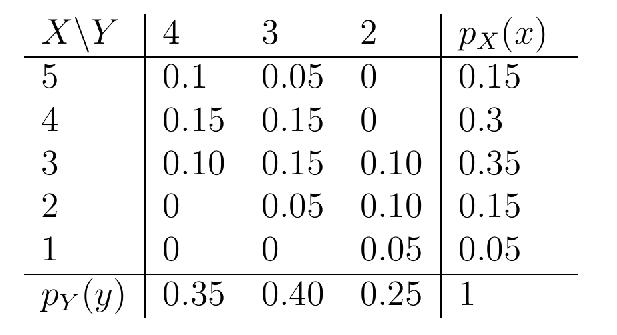
\includegraphics[width=2in]{extab1.png}
	\end{center}
	Find $P(X|Y=4)$ for $X=3,4,5$
	
	\item %Finan 43.5
	
	 Two dice are rolled. Let $X$ and $Y$ denote,
	 respectively, the largest and
	smallest values obtained. Compute the conditional mass function of $Y$ given
	$X = x$, for $x = 1, 2, \ldots, 6$. Are $X$ and $Y$ independent?
	
	\item %finan 43.6
	Let $X$ and $Y$ be discrete random variables with joint pmf
	$$f_{XY}(x,y) = \dfrac{n! y^x(p/e)^y(1-p)^{n-y}}{y!(n-y)x!}
	\qquad y=0,1,\ldots,n; x=0,1,\ldots$$
	\begin{enumerate}
		\item Find $f_Y(y)$
		\item Find $f_{X|Y}(x|Y=y)$
		\item Are $X$ and $Y$ independent? Why?
	\end{enumerate}

	\item %finan 43.8
	Let $X$ and $Y$ be discrete random variables with joint pmf
	$$f_{XY} = c(1-2^{-x})^y\qquad 0\leq x \leq N-1, y\geq 0$$
	\begin{enumerate}
		\item Find $c$
		\item Find $f_X(x)$
		\item Find $f_{Y|X}(y|x)$
	\end{enumerate}

	\item %finan 43.12
	Suppose that discrete random variables $X$ and $Y$ each take only the values 0
	and 1. It is known that $P(X = 0|Y = 1) = 0.6$ and $P(X = 1|Y = 0) = 0.7$.
	Is it possible that $X$ and $Y$ are independent? Justify your conclusion.
	
	\item %finan 43.15
	Let $X$ be the annual number of hurricanes hitting Florida, and let $Y$ be
	the annual number of hurricanes hitting Texas. $X$ and $Y$ are independent
	random variables with pmf:
	\begin{eqnarray*}
		f(x) &=& \dfrac{1.7^x}{x!}e^{-1.7} \qquad x\geq 0 \\
		g(y) &=& \dfrac{2.3^y}{y!}e^{-2.3} \qquad y\geq 0
	\end{eqnarray*}
	respective means 1.70 and 2.30.
	Calculate $\Pr[X − Y=k |X + Y = 3]$ for all $k$ in the 
	domain of $X-Y$.
	
	\item %finan 43.18
	A box contain 4 reds, 3 whites and 2 blues. A random sample of 3 balls is
	chosen. Let $R$ and $W$ be the number of red and white balls chosen. What is
	the conditional probability of $W = 2$ given that $R = 1$?
	
	\item %finan 43.21
	The probability of $x$ losses occurring in year $1$ is 
	$(0.5)^{x+1} , \qquad x = 0, 1, 2,\ldots$
	The probability of $y$ losses in year 2 given $x$ losses in year 1 is given by the table:
	\begin{center}
	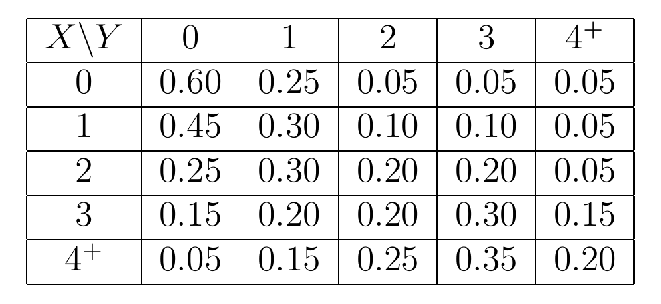
\includegraphics[width=2in]{extab2.png}
	\end{center}	
	Calculate the probability of exactly 2 losses in 2 years.
	
	\item %finan 43.22
	A flood insurance company determines that $N$, the number of claims received
	in a month, is a random variable with $\Pr[N=n] = \dfrac{2}{3^{n+1}}$ 
	for non-negative integers $n$.
	The numbers of claims received in different months are mutually independent. Calculate the probability that more than three claims will be received
	during a consecutive two-month period, given that fewer than two claims
	were received in the first of the two months.
	
\end{enumerate}
\end{exercises}

%--------------------------------------------------------------
%--------------------------------------------------------------
%--------------------------------------------------------------
\section{Continuous Random Variables}
The concepts we have studied so far with discrete random variables and mass functions transfer
almost immediately to continuous random variables, where sums are "replaced" with integrals. The fundamental underlying difference in interpretation is that a probability mass function becomes, in the continuous case, a probability \textit{density} function.

\subsection{Probability Density Functions}
\begin{definition}
Let $X$ be a random variable. A function $f(x)$ from the domain of $X$ into $\RR$ is a \textit{probability density function} (pdf) if it satisfies the following
\begin{enumerate}
    \item $f(x) \geq 0$ for all $x$ in the domain of $f$
    \item $\Pr[x \in A] = \Pr[A] = \int_A f(x) \dx$ gives the probability
    that the random variable $X$ dispenses an element of the set $A$
    \item $\int_\mathcal{A} f(x) \dx = 1$ where $\mathcal{A}$ is the entire domain
    of the random variable $X$
\end{enumerate}
\end{definition}
%
Notice the third property above is general enough to allow integrating over any measurable set. Indeed, in almost
all cases we will encounter problems where we integrated over contiguous sets such as intervals. In this case we can write
$$\Pr[a < X < b] = \int_a^b f(x) \dx.$$
\begin{example}
    Let $f(x)=e^{-x}$ be the pdf of $X$ defined over $\mathcal{A} = \{x | 0<x<\infty\}$. Find
    \begin{enumerate}
        \item $\Pr[0<X<1]$
        \item $\Pr[X>10]$
        \item $\Pr[X \dsp 3]$
    \end{enumerate}
\end{example}
\begin{solution}
Each of the probabilities becomes an integral computation.
    \begin{enumerate}
        \item $\displaystyle \int_0^1 f(x)\dx = 1-\dfrac{1}{e}$
        \item $\displaystyle \int_{10}^\infty f(x)\dx = \dfrac{1}{e^{10}}$
        \item $\displaystyle \int_3^3 f(x)\dx = 0 $ even though $f(3) = \dfrac{1}{e^3}$
    \end{enumerate}
In the last item notice a fundamental difference between probability density functions and probability mass functions.
In the case of a pdf, the value of $f(x)$ at any point $x$ does \textit{not} give a probability but rather a density.
The probability that $X \dsp k$ for any constant $k$ is 0 whenever $X$ is a continuous random variable. We can determine
a non-zero probability that $X$ is within a given interval of $k$ by integrating the density function and determining a probability "mass" near the point.
\end{solution}

\begin{example}
Let $X$ be a random variable on $mathcal{A} = \{x \, | \, 0<x<1\}$ with pdf $f(x) = cx^2$. Determine $c$.
\end{example}
\begin{solution}
Since $f$ is a pdf
\begin{eqnarray*}
    \int_0^1 f(x) \dx &=& 1 \\
    \int_0^1 cx^2 \dx&=& 1 \\
    \dfrac{c}{3} &=& 1 \\
    c &=& 3
\end{eqnarray*}
\end{solution}

\subsection{Cumulative Distribution Function}
\begin{definition}
The \textit{cumulative distribution function} (cdf) of a random variable $X$ with pdf $f$ is defined as
$$F(x) = \Pr[X < x] = \int_{-\infty}^x f(t) \dt$$
in which it is assumed $f(x)$ is defined over all the reals, with positive density in the support of $X$ and zero density
elsewhere.
\end{definition}

\begin{example}
Find the CDF for each of the following PDFs.
\begin{enumerate}
    \item $f(x) = \dfrac{1}{\pi(1+x^2)}$ where $x \in \RR$
    \item $f(x) = \dfrac{e^{-x}}{(1+e^{-x})^2}$ where $x \in \RR$
    \item $f(x) = \dfrac{a-1}{(1-x)^a}$ where $0<x<\infty$
    \item $f(x) = k\alpha x^{\alpha-1}e^{-kx^{\alpha}}$ for $ 0<x<\infty,\,k<0,\,\alpha>0$
\end{enumerate}
\begin{solution}
The CDFs are found by integrating

\begin{enumerate}
    \item $F(x) = \dfrac{1}{\pi}\arctan x + \dfrac{1}{2}$
    \item $F(x) = \dfrac{1}{1+e^{-x}}$
    \item $F(x) = 
        \begin{cases}
            1 - \dfrac{1}{(1+x)^{\alpha-1}} & x>0\\
            0 & x \leq 0
        \end{cases}$
    \item $F(x) =
        \begin{cases}
            1 - e^{-kx^\alpha} & x>0 \\
            0 & x \leq 0
        \end{cases}$
\end{enumerate}
Where in the last two we are careful to set the lower bound of integration to 0, given the definition of $f(x)$.
\end{solution}
\end{example}
\subsection{Joint Density Functions: Cumulative, Marginal and Conditional}
Given two random variables $X,Y$ over continuous spaces, the joint pdf can be defined
analogously to a discrete joint pmf.
\begin{definition}
Given continuous random variables $X,Y$, the function $f(x,y)$ is a \textit{joint pdf} for $X,Y$
if 
\begin{enumerate}
    \item $f(x,y) \geq 0$ for all $x,y \in \RR^2$
    \item $\displaystyle\int\!\!\int_{\RR^2} f(x,y) \dx \dy  = 1$
\end{enumerate}
\end{definition}
Similarly we can extend the definitions already given for cumulative, marginal, and conditional distributions
\begin{definition}
    Given two random variables $X,Y$
    \begin{itemize}
        \item The \textbf{cumulative distribution function} $F(x,y)$ is defined
        $$F(x,y) = \Pr[X<x,Y<y] = \int_{-\infty}^y \!\! \int_{-\infty}^x f(u,v) \du \dv$$
        \item The \textbf{marginal distribution function} $f_X(x)$ is computed
        by integrating out the $y$ values
        $$ f_X(x) = \int_{-\infty}^{\infty} f(x,y) \dy $$
        \item The \textbf{condition distribution of $X$ given $Y$} is computed by dividing the 
        joint pdf by the marginal of $Y$:
        $$f_{X|y}(x|y) = \dfrac{f(x,y)}{f_Y(y)} = \dfrac{f(x,y)}{\int_{-\infty}^{\infty} f(x,y) \dx }$$
    \end{itemize}
\end{definition}
\begin{example}
Let $f(x,y) = x+y$ be the pdf for $X,Y$ over the square $0<x<1, 0<y<1$. Determine the 
CDF $F(x,y)$.
\end{example}
\begin{solution}
First note that the definition of $F$ will have 5 pieces: when $x<0$ or $y<0$, when $x>1,0<y<1$,
when $y>1, 0<x<1$, when $0<x<1, 0<y<1$ and when $x>1,y>1$. In the first case there is no probability density so $F(x,y) = 0$. To handle the other cases we will first compute $G(x,y)
 = \int_0^y\int_0^x f(x,y) \dx \dy$ so
 $$G(x,y) = \dfrac{xy}{2}(x+y), \; x>0, y>0.$$
 To solve the problem, notice that $F(x,y) = G(x,y)$ when both arguments are within the unit square. But if $x>1$, then $F(x,y) = G(1,y)$ because $\Pr[X>1] = 0$. Similarly if $y>1$,
 $F(x,y) = G(x,1)$. And finally if $x>1,y>1$ then $F(x,y) = G(1,1) = 1$. So
 $$F(x,y) = 
    \begin{cases}
        \dfrac{xy}{2}(x+y) & 0<x<1, 0<y<1 \\[4ex]
        \dfrac{y}{2}(1+y) & 0<y<1, x>1 \\[4ex]
        \dfrac{x}{2}(x+1) & 0<x<1, y>1 \\[4ex]
        1 & x>1, y>1 \\
        0 & \mbox {otherwise}
    \end{cases}$$
\end{solution}
\subsection{Mixed Distributions}
\subsection{Functions of Random Variables}

\begin{exercises}
\begin{enumerate}
	\item Let $f(x) = \dfrac{c}{(x+1)^3}$ be a pdf for $x \geq 0$. Determine the value of $c$ %finan 28.1
	
	\item The lifetime $X$ of a battery (in hours)
	has a density function given by
	$$f(x) = 
	\begin{cases}
		2x & 0 \leq x < \frac12 \\
		\frac34 & 2 < x < 3 
	\end{cases}$$
	Find the probability that a battery will last for more than 15 minutes. %finan 28.4
	
	\item %finan 28.5
	Let $F(x)$ be a CDF defined below.
	$$F(x) = 
	\begin{cases}
		0	& x<0\\
		x/2 	& 0 \leq x < 1 \\
		(x+2)/6	& 1 \leq x < 4 \\
		1		& x \geq 4
	\end{cases}$$
	Find the pdf $f(x)$ corresponding to $F$.
	
	\item %finan 28.7
	A mixed random variable $X$ has CDF
	$$F(x) = 
	\begin{cases}
	0		& x<0\\
	\dfrac{e^x}{e^x+1}	& x \geq 0
	\end{cases}$$
	\begin{enumerate}
		\item Find the pdf
		\item Find $\Pr[0 < X \leq 1]$
	\end{enumerate}
	
	\item %finan 28.24
	Let $X$ be a continuous random variable with probability density function
		$$f(x) = \lambda e^{-\lambda x}$$
		where $\lambda > 0$. Let $Y$ be the smallest integer greater than or equal to $X$.
	Determine the probability density function of $Y$.
	
	\item %finan 28.14
	Let $X$ have pdf $$f(x) = \dfrac{3x^2}{\theta^3} \;
	0 < x < \theta.$$ If $\Pr[X>1] = \frac78$, find $\theta$
	
	\item %finan 28.9
	The loss due to a fire in a commercial building is modeled by a random
	variable $X$ with density function
	$$f(x) = 0.005(20-x) \qquad 0<x<20$$
	Given that a fire loss exceeds 8, what is the probability that
	it exceeds 16?
	
	\item %finan 28.12
	An insurance company insures a large number of homes. The insured value,
	$X$, of a randomly selected home is assumed to follow a distribution with
	density function
	$$f(x) = 3x^{-4} \qquad x>1$$
	Given that a randomly selected home is insured for at least
	1.5, what is the probability that it is insured for less than 
	2?
	
	\item %finan 28.15
	Let $X$ be a continuous random variable with density function
	$$f(x) = \dfrac{|x|}{10} \qquad -2 \leq x \leq 4$$
	Calculate $\displaystyle \int_{-\infty}^\infty xf(x)\dx$.
	
	\item %finan 28.23
	A large university will begin a 13-day period during which students may register for that semester’s courses. Of those 13 days, the number of elapsed days
	before a randomly selected student registers has a continuous distribution
	with density function $f(t)$ that is symmetric about $t = 6.5$ and proportional
	to $\dfrac{1}{t+1}$
	between days 0 and 6.5.
	A student registers at the 60th percentile of this distribution. Calculate the
	number of elapsed days in the registration period for this student.
	
\end{enumerate}
\end{exercises}
\end{document}











































